
\subsection*{1.}

\(f(x) = 4x^3 - 48x^2 + 144x\).

\paragraph{a.} La fonction polynôme \( f \) est dérivable sur \( \mathbb{R} \) et sur cet intervalle :
\[
f'(x) = 12x^2 - 96x + 144 = 12x^2 - 12 \times 8x + 12 \times 12 = 12(x^2 - 8x + 12).
\]

\paragraph{b.} Pour le trinôme \( x^2 - 8x + 12 \), on a :
\[
\Delta = 64 - 48 = 16 = 4^2.
\]

Il y a donc deux racines :
\[
x_1 = \dfrac{8 + 4}{2} = 6 \quad \text{et} \quad x_2 = \dfrac{8 - 4}{2} = 2.
\]

On sait que le trinôme est positif sauf sur l'intervalle \( ]2\,;\,6[ \) où \( f'(x) < 0 \).

La fonction est donc croissante sauf sur l'intervalle \( ]2\,;\,6[ \).

Avec \( f(2) = 128 \) et \( f(6) = 0 \), on a le tableau de variations suivant :
\begin{center}
\begin{tikzpicture}
\tkzTabInit[lgt=3, espcl=3.5]{$x$ / 1, {Signe de $f'(x)$} / 1, {$f$} / 2}{${-\infty}$, ${2}$, ${6}$, ${+\infty}$}
\tkzTabLine{,+,0,-,0,+,}
\tkzTabVar{-/{$$},+/{$128$},-/{$0$},+/{$$}}{/}
\end{tikzpicture}
\end{center}

\subsection*{2.}

\paragraph{a.} La boîte a une base carrée de \( 12 - 2 \times 1 = 10 \) de côté et une hauteur de 1. Son volume est donc égal à :
\[
V(1) = 1 \times 10^2 = 100 \, \text{cm}^3.
\]

\paragraph{b.} En général, pour \( 0 \leqslant x \leqslant 6 \), la boîte a une base carrée de \( 12 - 2x \) de côté et une hauteur de \( x \). Son volume est donc égal à :
\[
V(x) = (12 - 2x)^2 \times x = x \times (144 + 4x^2 - 48x) = 4x^3 - 48x^2 + 144x = f(x).
\]

\paragraph{c.} On a vu que \( f \) a un maximum : \( f(2) = 128 \).

Le volume maximal \( 128 \, \text{cm}^3 \) est obtenu pour \( x = 2 \, \text{cm} \).

